\documentclass[12pt]{article}
%\usepackage[document]{ragged2e}
\usepackage{array, amssymb, amsthm, linguex, enumerate, amsmath, physics, enumitem, xcolor, graphicx, xparse}
\let\fg\undefined %remove linguex/siunitx naming clash
\usepackage[english]{babel}
\usepackage[letterpaper,top=2cm,bottom=2cm,left=3cm,right=3cm,marginparwidth=1.75cm]{geometry}
\usepackage[colorlinks=true, allcolors=blue]{hyperref}
\usepackage[group-separator={,}]{siunitx} %\num{12345} -> "12,345"
\usepackage{fancyhdr}
\usepackage{notomath}
\usepackage[T1]{fontenc}
\usepackage{multicol}
\usepackage{mathtools}

%Number sets
\newcommand{\R}{\mathbb{R}}
\newcommand{\C}{\mathbb{C}}
\newcommand{\N}{\mathbb{N}}
\newcommand{\F}{\mathbb{F}}
\renewcommand{\Re}{\operatorname{Re}}
\renewcommand{\Im}{\operatorname{Im}}
\renewcommand{\L}[1]{\mathcal{L}\left({#1}\right)} %Linear Map

\newcommand{\pmp}{\,\pm\,} %add small extra space to \pm

\NewDocumentCommand{\ceil}{ s m }{% ceiling brackets
    \IfBooleanTF{#1}%
    {\lceil #2 \rceil}% starred: no-autosizing
    {\left\lceil #2 \right\rceil}% unstarred: autosizing
}

\NewDocumentCommand{\ceiling}{ s m }{% ceiling brackets
    \IfBooleanTF{#1}%
    {\lceil #2 \rceil}% starred: no-autosizing
    {\left\lceil #2 \right\rceil}% unstarred: autosizing
}

\NewDocumentCommand{\floor}{ s m }{% floor brackets
    \IfBooleanTF{#1}%
    {\lfloor #2 \rfloor}% starred: no-autosizing
    {\left\lfloor #2 \right\rfloor}% unstarred: autosizing
}

\NewDocumentCommand{\pars}{ s m }{% parenthesis
    \IfBooleanTF{#1}%
    {( #2 ) }% starred: no-autosizing
    {\left( #2 \right) }% unstarred: autosizing
}

\NewDocumentCommand{\inner}{ s m }{% inner product
    \IfBooleanTF{#1}%
    {\langle #2 \rangle}% starred: no-autosizing
    {\left\langle #2 \right\rangle}% unstarred: autosizing
}

\NewDocumentCommand{\innerconj}{ s m }{% inner product
    \IfBooleanTF{#1}%
    {\overline{\langle #2 \rangle}}% starred: no-autosizing
    {\overline{\left\langle #2 \right\rangle}}% unstarred: autosizing
}

\NewDocumentCommand{\brac}{ s m }{% brackets
    \IfBooleanTF{#1}%
    {[#2] }% starred: no-autosizing
    {\left[ #2 \right] }% unstarred: autosizing
}

%default latex bracket size naming
\newcommand{\biggbrac}[1]{\bigg[ {#1} \bigg] }
\newcommand{\bigbrac}[1]{\big[ {#1} \big] }
\newcommand{\Bigbrac}[1]{\Big[ {#1} \Big] }


\RenewDocumentCommand{\over}{ s m }{% fraction 1/arg
    \IfBooleanTF{#1}%
    {\dfrac{1}{#2}}% starred: dfrac
    {\frac{1}{#2}}% unstarred: normal frac
}

\NewDocumentCommand{\pover}{ s m }{% parenthesis around fraction (1/arg)
    \IfBooleanTF{#1}%
    {\left(\dfrac{1}{#2}\right)}% starred: dfrac
    {\left(\frac{1}{#2}\right)}% unstarred: normal frac
}

\NewDocumentCommand{\pfrac}{ s m m}{% parenthesis around fraction (arg1/arg2)
    \IfBooleanTF{#1}%
    {\left( \dfrac{{#2}}{{#3}} \right)}% starred: dfrac
    {\left( \frac{{#2}}{{#3}} \right)}% unstarred: normal frac
}


\newcommand{\Xbar}{\bar{X}}
\newcommand{\Ybar}{\bar{Y}}
\newcommand{\xbar}{\bar{x}}
\newcommand{\ybar}{\bar{y}}
\newcommand{\xstar}{x^{\ast}}

\newcommand{\limn}{\lim_{n\to\infty}}

\newcommand{\gammaDist}[2]{\operatorname{Gamma} \left( {#1},{#2} \right)} %gamma distribution
\NewDocumentCommand{\normalDist}{s g g}{ %normal distibution
    \IfBooleanTF{#1} { % starred, no autosizing parenthesis
      \IfNoValueTF{#2}{
          N (\mu,\, \sigma^2 ) %\normalDist* "default" normal distribution N(\mu, \sigma^2)
        } {
            \IfNoValueTF{#3}{N (#2)}{} %\normalDist{arg} --> N(arg)
        }
      \IfNoValueTF{#3}{}{N ( #2, #3 )}  %\normalDist*{arg1}{arg2} --> N(arg1,arg2)
    }  % else (unstarred) autosize parenthesis
    {
        \IfNoValueTF{#2}{
            N \left(\mu,\, \sigma^2 \right) %\normalDist "default" normal distribution N(\mu, \sigma^2)
        } {
            \IfNoValueTF{#3}{N \left(#2\right)}{} %\normalDist{arg} --> N(arg)
        }
        \IfNoValueTF{#3}{}{N \left( #2, #3 \right)} %\normalDist{arg1}{arg2} --> N(arg1,arg2)
    }
}



%colors
\definecolor{ggreen}{RGB}{0, 127, 0}
\definecolor{dgray}{RGB}{63,63,63}
\definecolor{neonorange}{RGB}{255,47,0}
\definecolor{mygray}{rgb}{0.5,0.5,0.5}
\definecolor{eblue}{RGB}{0,74,127}
\newcommand{\red}[1]{\color{red}{#1}\color{black}}
\newcommand{\green}[1]{\color{ggreen}{#1}\color{black}}
\newcommand{\blue}[1]{\color{blue}{#1}\color{black}}
\newcommand{\setRed}{\color{red}}
\newcommand{\setBlack}{\color{black}}
\newcommand{\setBlue}{\color{blue}}
\newcommand{\setGreen}{\color{ggreen}}



\newcommand{\thru}[1]{{#1}_1, \dots, {#1}_n}
\newcommand{\sumThru}[1]{{#1}_1 + \cdots + {#1}_n}
\newcommand{\yn}{Y_1, \dots, Y_n} % Y_1, ..., Y_n
\newcommand{\xn}{X_1, \dots, X_n} % Y_1, ..., Y_n

%hats and tildes
\newcommand{\that}{\widehat{\theta}} % theta hat
\newcommand{\phat}{\widehat{p}} % p hat
\newcommand{\qhat}{\widehat{q}} % p hat
\newcommand{\psihat}{\widehat{\psi}} % psi hat
\newcommand{\Psihat}{\widehat{\Psi}} % Psi hat
\newcommand{\ptilde}{\widetilde{p}} % psi tilde
\newcommand{\Psitil}{\widetilde{\Psi}} % Psi tilde
\newcommand{\betah}{\widehat{\beta}} % beta hat
\newcommand{\bat}{\widehat{\beta}} % beta hat
\newcommand{\xhat}{\widehat{x}} % beta hat
\newcommand{\yhat}{\widehat{y}} % beta hat

%2x2 matrix shortcuts
\newcommand{\detx}[4]{\begin{vmatrix}{#1} & {#2}\\{#3}&{#4}\end{vmatrix}} % 2x2 determinant
\newcommand{\dety}[9]{\begin{vmatrix}{#1} & {#2} & {#3} \\{#4}&{#5}&{#6}\\ {#7} & {#8} & {#9}\end{vmatrix}} % 3x3 determinant
\newcommand{\bmaty}[9]{\begin{bmatrix}{#1} & {#2} & {#3} \\{#4}&{#5}&{#6}\\ {#7} & {#8} & {#9}\end{bmatrix}} % 3x3 matrix
\newcommand{\bmat}[4]{\begin{bmatrix}{#1} & {#2}\\{#3}&{#4}\end{bmatrix}} % 2x2 matrix brackets
\renewcommand{\pmat}[4]{\begin{pmatrix}{#1} & {#2}\\{#3}&{#4}\end{pmatrix}} % 2x2 matrix parenthesis

%remove any enumerate/itemize indent temporarily
\makeatletter   %% <- make @ usable in macro names
\newcommand*\notab[1]{%
  \begingroup   %% <- limit scope of the following changes
    \par        %% <- start a new paragraph
    \@totalleftmargin=0pt \linewidth=\columnwidth
    %% ^^ let other commands know that the margins have been reset
    \parshape 0
    %% ^^ reset the margins
    #1\par      %% <- insert #1 and end this paragraph
  \endgroup
}
\makeatother    %% <- revert @


\newcommand{\dimrange}[1]{\operatorname{dim}\operatorname{range}{#1}} % dimrange
\newcommand{\dimnull}[1]{\operatorname{dim}\operatorname{null}{#1}} % dimnull
\newcommand{\range}[1]{\operatorname{range}{#1}} %range
\newcommand{\nullspace}{\operatorname{null}} %null

% polynomial notation
\NewDocumentCommand{\poly}{ s g g }{%
    \IfBooleanTF{#1} {
        \IfNoValueTF{#2} {
            \mathcal{P}(\mathbb{R})
        } {
            \mathcal{P}_{#2}(\mathbb{R})
        }
    } {
        \IfNoValueTF{#3} {
            {\mathcal{P}(#2)}
        } { %else
            {\mathcal{P}_{#2}(#3)}
        }
    }
}

\NewDocumentCommand{\bias}{ s m }{% bias(arg)
    \IfBooleanTF{#1}%
    {\operatorname{bias}(#2)}% starred: no autosizing
    {\operatorname{bias}\left(#2\right)}% unstarred: autosizing
}

\NewDocumentCommand{\MSE}{ s m }{% MSE(arg)
    \IfBooleanTF{#1}%
    {\operatorname{MSE}(#2)}% starred: no autosizing
    {\operatorname{MSE}\left(#2\right)}% unstarred: autosizing
}

\NewDocumentCommand{\Var}{ s m }{% variance with parenthesis V(arg)
    \IfBooleanTF{#1}%
    {\operatorname{Var}(#2)}% starred: no autosizing
    {\operatorname{Var}\left(#2\right)}% unstarred: autosizing
}

\NewDocumentCommand{\Varb}{ s m }{% variance with brackets V[arg]
    \IfBooleanTF{#1}%
    {\operatorname{Var}[\,#2\,]}% starred: no autosizing
    {\operatorname{Var}\left[\,#2\,\right]}% unstarred: has autosizing
}

\NewDocumentCommand{\Vb}{ s m }{% another renaming of variance with brackets V[arg]
    \IfBooleanTF{#1}%
    {\operatorname{Var}[\,#2\,]}% starred: no autosizing
    {\operatorname{Var}\left[\,#2\,\right]}% unstarred: has autosizing
}

\NewDocumentCommand{\E}{ s m }{% expectation with parenthesis E(arg)
    \IfBooleanTF{#1}%
    {\operatorname{E}(#2)}% starred: no autosizing
    {\operatorname{E}\left(#2\right)}% unstarred: has autosizing
}

\NewDocumentCommand{\Eb}{ s m }{% expectation with brackets E[arg]
    \IfBooleanTF{#1}%
    {\operatorname{E}[#2]}% starred: no autosizing
    {\operatorname{E}\left[#2\right]}% unstarred: has autosizing
}

\RenewDocumentCommand{\P}{ s m }{% probability with parenthesis Pr(arg)
    \IfBooleanTF{#1}%
    {\Pr (#2) }% starred: no autosizing
    {\Pr \left( #2 \right) }% unstarred: has autosizing
}

\NewDocumentCommand{\prob}{ s m }{% probability with parenthesis Pr(arg)
    \IfBooleanTF{#1}%
    {\Pr (#2) }% starred: no autosizing
    {\Pr \left( #2 \right) }% unstarred: has autosizing
}

\NewDocumentCommand{\eff}{ s m }{% efficiency with parenthesis eff(arg)
    \IfBooleanTF{#1}%
    {\operatorname{eff}(#2)}% starred: no autosizing
    {\operatorname{eff}\left(#2\right)}% unstarred: has autosizing
}

%vertical vector of up to 8 elements
\NewDocumentCommand\vvec{s m g g g g g g g}{%
    \IfBooleanTF{#1} {
        \begin{bmatrix}% if starred use brackets
            \IfNoValueTF{#2}{}{#2}
            \IfNoValueTF{#3}{}{\\#3}
            \IfNoValueTF{#4}{}{\\#4}
            \IfNoValueTF{#5}{}{\\#5}
            \IfNoValueTF{#6}{}{\\#6}
            \IfNoValueTF{#7}{}{\\#7}
            \IfNoValueTF{#8}{}{\\#8}
        \end{bmatrix}
    }  % else (unstarred) use parethesis
    {
        \begin{pmatrix}%
            \IfNoValueTF{#2}{}{#2}
            \IfNoValueTF{#3}{}{\\#3}
            \IfNoValueTF{#4}{}{\\#4}
            \IfNoValueTF{#5}{}{\\#5}
            \IfNoValueTF{#6}{}{\\#6}
            \IfNoValueTF{#7}{}{\\#7}
            \IfNoValueTF{#8}{}{\\#8}
        \end{pmatrix}
    }
}
\def\Cov{\operatorname{Cov}} %Covariance
\def\df{\text{df}} %degrees of freedom

\NewDocumentCommand{\example}{ s g }{% Example header
    \IfBooleanTF{#1}%
    {\vspace{0.1in}}% starred: 0.1in
    {\vspace{0.2in}}% unstarred: 0.2in
    \IfNoValueTF{#2} {\noindent\textbf{\color{eblue} Example: }}{\noindent\textbf{\color{eblue} Example (#2): }}
}
\NewDocumentCommand{\disc}{ s }{% Discussion header
    \IfBooleanTF{#1}%
    {\vspace{0.1in}\noindent\textbf{Discussion: } }% starred: 0.1in
    {\vspace{0.2in}\noindent\textbf{Discussion: } }% unstarred: 0.2in
}
\NewDocumentCommand{\defn}{ s }{% Definition header
    \IfBooleanTF{#1}%
    {\vspace{0.1in}\noindent\textbf{\color{neonorange} Definition: } }% starred: 0.1in
    {\vspace{0.2in}\noindent\textbf{\color{neonorange} Definition: } }% unstarred: 0.2in
}
\NewDocumentCommand{\reason}{ s }{% Reason header
    \IfBooleanTF{#1}%
    {\vspace{0.1in}\noindent\textbf{Reason:} }% starred: 0.1in
    {\vspace{0.2in}\noindent\textbf{Reason:} }% unstarred: 0.2in
}
\NewDocumentCommand{\recall}{ s }{% Recall header
    \IfBooleanTF{#1}%
    {\vspace{0.1in}\noindent\textit{Recall:} }% starred: 0.1in
    {\vspace{0.2in}\noindent\textit{Recall:} }% unstarred: 0.2in
}
\NewDocumentCommand{\remark}{ s }{% Remark header
    \IfBooleanTF{#1}%
    {\vspace{0.1in}\noindent\textit{Remark:} }% starred: 0.1in
    {\vspace{0.2in}\noindent\textit{Remark:} }% unstarred: 0.2in
}

\NewDocumentCommand{\soln}{ s }{% Remark header
    \IfBooleanTF{#1}%
    {\vspace{0.1in}\noindent\textbf{Solution: } }% starred: 0.1in
    {\vspace{0.2in}\noindent\textbf{Solution: } }% unstarred: 0.2in
}

\newcommand{\proj}[2]{\operatorname{proj}_{{#1}}{#2}} %projection
\newcommand{\wideand}{\qquad \text{and} \qquad}

\newcommand{\bu}[1]{\textbf{\underline{{#1}}} } %bold underline
\newcommand{\boldit}[1]{\textbf{\textit{{#1}}} } %bold italix

% put actual quotation marks "around something"
\newcommand{\say}[1]{\textquotedblleft{#1}\textquotedblright}

% max{arg} and min{arg}
\renewcommand{\max}[1]{\operatorname{max}\left\{ #1 \right\}}
\renewcommand{\min}[1]{\operatorname{min}\left\{ #1 \right\}}

\newcommand{\Span}[1]{\operatorname{span}\left\{ #1 \right\}}

%Create a new vspace line no indent
\newcommand{\nl}{\vspace{0.1in}\noindent}
\newcommand{\nnl}{\vspace{0.2in}\noindent}
\newcommand{\nnnl}{\vspace{0.3in}\noindent}
\textwidth=7.02in
\hoffset=-.425in

\setcounter{MaxMatrixCols}{20}
\begin{document}
\pagestyle{fancy}
\fancyhf{}
\fancyhead[RO]{Matthew Wilder}
\fancyhead[LO]{MTH 427 - Homework \#3}
\fancyfoot[CO]{Page \thepage}

\noindent MTH 427 - Spring 2023
\\Assignment \#3
\\Due: Monday, March 6th 2023 (11:59PM)


\begin{enumerate}
\item For any random variables $X$, $Y$ and any constants $a, b, c$ and $d$,
\\show that $\Cov(a+bX, c+dY) = bd \Cov(X,Y)$.

\begin{proof}
    \begin{align*}
        \Cov(a+bX, c+dY) &= \Eb{(a+bX)(c+dY)} - \Eb{a+bX}\Eb{c+dY}\\
        &= \Eb{ac+adY+bcX+bdXY} - \pars{\Eb{a}+\Eb{bX}}\pars{\Eb{c}+\Eb{dY} }\\
        &= ac + ad\Eb{Y} + bc\Eb{X} + bd\Eb{XY} - \pars{a + b\Eb{X}}\pars{c + d\Eb{Y}}\\
        &= ac + ad\Eb{Y} + bc\Eb{X} + bd\Eb{XY} - \pars{ac + ad\Eb{Y} + bc\Eb{X} + bd\Eb{X}\Eb{Y}}\\
        &= bd\Eb{XY} - bd\Eb{X}\Eb{Y} \tag{\say{Lots of killing} - McAsey}\\
        &= bd\pars{\Eb{XY} - \Eb{X}\Eb{Y}}\\
        &= bd \Cov(X,Y)
    \end{align*}
\end{proof}
\item Is the plant density of a species related to the altitude at which data are collected? Let $Y$ denote the species density and $X$ denote the altitude. A fit of a simple linear regression model using 14 observations yielded $\yhat = 21.6 - 7.79x$ and $r^2 = 0.61$.
\begin{enumerate}
\item What is the value of the correlation coefficient $r$?

\soln* $r^2 = 0.61 \iff r = \pm 0.781$, but because $\bat_1 < 0$ then $r = -0.781$.
\item If $\that_1$ and $\that_2$ are independent, how should $\alpha$ be chosen in order to minimize the variance of $\that_3$?

\soln* First derive the general form of the variance of the estimator $\that_3$. That is, 
\begin{align*}
    \Varb*{\that_3} &= \Varb*{\alpha \that_1 + (1-\alpha)\that_2} \tag{substitute}\\
    &= \alpha^2 \Varb*{\that_1} + (1-\alpha)^2 \Varb*{\that_2} + 2\alpha(1-\alpha) \Cov(\that_1, \that_2) \tag{formula}\\
    &= \alpha^2 \Varb*{\that_1} + (1-\alpha)^2 \Varb*{\that_2} \tag{By independence hypothesis}\\
    &= \alpha^2 {\sigma_1}^2 + (1-\alpha)^2 {\sigma_2}^2 \tag{substitute}
\end{align*}
Using the first derivative test wrt $\alpha$, 
$\displaystyle \pdv{\alpha} \pars{\alpha^2 {\sigma_1}^2 + (1-\alpha)^2 {\sigma_2}^2} = 2\alpha({\sigma_1}^2 + {\sigma_2}^2) + 2{\sigma_2}^2$. Setting this equal to 0 and solving for $\alpha$ yields 
$\alpha = \dfrac{{\sigma_2}^2}{{\sigma_1}^2+{\sigma_2}^2}$.

\end{enumerate}
\newpage
\item Refer to exercise 11.3. Fit the model suggested there by use of matrices. 

\soln*
\begin{center}
    \begin{tabular}{l|ccccc}
         y & 3 & 2 & 1 & 1 & 0.5\\
         \hline
         x & -2 & -1 & 0 & 1 & 2\\
    \end{tabular}
\end{center}

$$
X = \begin{bmatrix}
	1 & -2\\
	1 & -1\\
	1 & 0\\
	1 & 1\\
	1 & 2\\
\end{bmatrix}
, \quad X^T =
\begin{bmatrix}
	1 & 1 & 1 & 1 & 1\\
	-2 & -1 & 0 & 1 & 2\\
\end{bmatrix}
, \quad Y=
\begin{bmatrix}
	3\\
	2\\
	1\\
	1\\
	0.5\\
\end{bmatrix}
$$
$$
X^TX = \begin{bmatrix}
	5 & 0\\
	0 & 10\\
\end{bmatrix}, \qquad (X^TX)^{-1} = \begin{bmatrix}
	\frac15 & 0\\
	0 & \frac{1}{10}\\
\end{bmatrix}
$$
$$
X^TY = \begin{bmatrix}
	7.5\\
	-6\\
\end{bmatrix}
$$
$$
\bat = (X^TX)^{-1}\cdot X^TY = \begin{bmatrix}
	\frac15 & 0\\
	0 & \frac{1}{10}\\
\end{bmatrix}
\begin{bmatrix}
	7.5\\
	-6\\
\end{bmatrix} = \begin{bmatrix}
	1.5\\
	-0.6\\
\end{bmatrix}
$$
$$\therefore \yhat = -0.6x + 1.5$$
\item \textbf{Exercise 1}

\nl This exercise relates to the \textbf{Auto} dataset, which can be found in Canvas. (This is part 2 of Additional exercise Homework \#2).

\textit{Note: Screenshots of code/outputs at end of problem}
\begin{enumerate}
\item Use the appropriate function in R to fit a quadratic model ($Y = \bat_0 + \bat_1 x + \bat_2 x^2 + \varepsilon$) with \textbf{mpg} as the response variable, and where \textbf{horsepower} and \textbf{horsepower$^2$} are the predictors.

\soln*
\begin{center}
    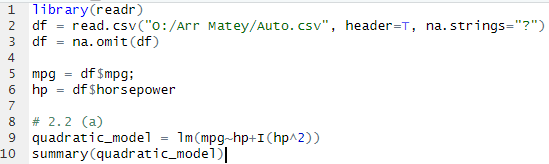
\includegraphics[width=5in]{img/a.PNG}
\end{center}

\item Write out the estimated model in equation form.

\soln*
$$\yhat(h) = 56.9000997 + -0.4661896 h + 0.0012305 h^2$$
\item Compute the covariance matrix for the linear regression coefficients estimated.

\soln*
\texttt{vcov(quadratic\_model)}
$$
\begin{bmatrix}
	3.2415366849 & -0.05493052 & 0.0002054469\\
	-0.0549305164 & 0.0009687418 & -3.734238 \cdot 10^{-6} \\
    0.0002054469 & -3.734238 \cdot 10^{-6} & 1.490252 \cdot 10^{-8}\\
\end{bmatrix}$$

\item 
Do the data present sufficient evidence to indicate curvature in the response function?
That is to test the hypotheses $H_0 : \bat_2 = 0$ vs $H_a : \bat_2 \neq 0$.
(Hint: you may use the $p$-value from your summary in part (a))

\soln*
Because $p = -2 \cdot 10^{-16} < 0.05 = \alpha$ we reject $H_0$ and conclude that there is evidence of curvature in the response function.
\item 
Based on the $R^2$ or Adjusted $R^2$, compare the fits of the quadratic model in part (a)
with the simple linear regression model (from Additional exercise of Homework \#2) where mpg
is the response variable and horsepower is the only predictor variable.

\soln*
In homework 2 the degree 1 polynomial estimate had an R-squared of $0.6059$. In the new model the $R^2 = 0.6876$ and adjusted $R^2 = 0.686$. The new second order term helps to explain approximately 13\% more of the variance $\pfrac{0.686}{0.6049}$.
\end{enumerate}

\begin{center}
    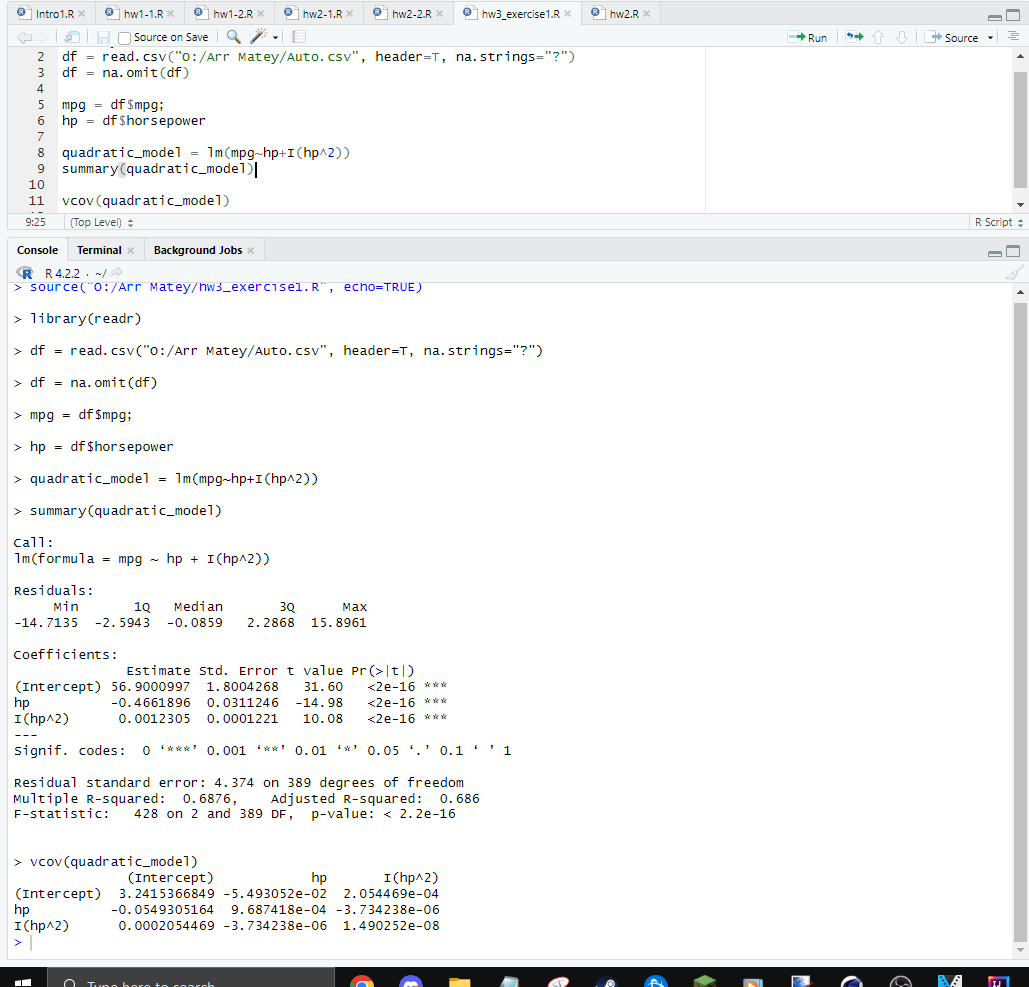
\includegraphics[width=6in]{img/ex1.PNG}
\end{center}
\item \textbf{Exercise 2}

\nl This question should be answered using the \textbf{Credit} dataset in Canvas.
\begin{enumerate}
\item 
Fit a multiple regression model to predict \green{Balance } using \blue{Income, Limit, Education,
and Rating.}

\soln* \begin{center}
    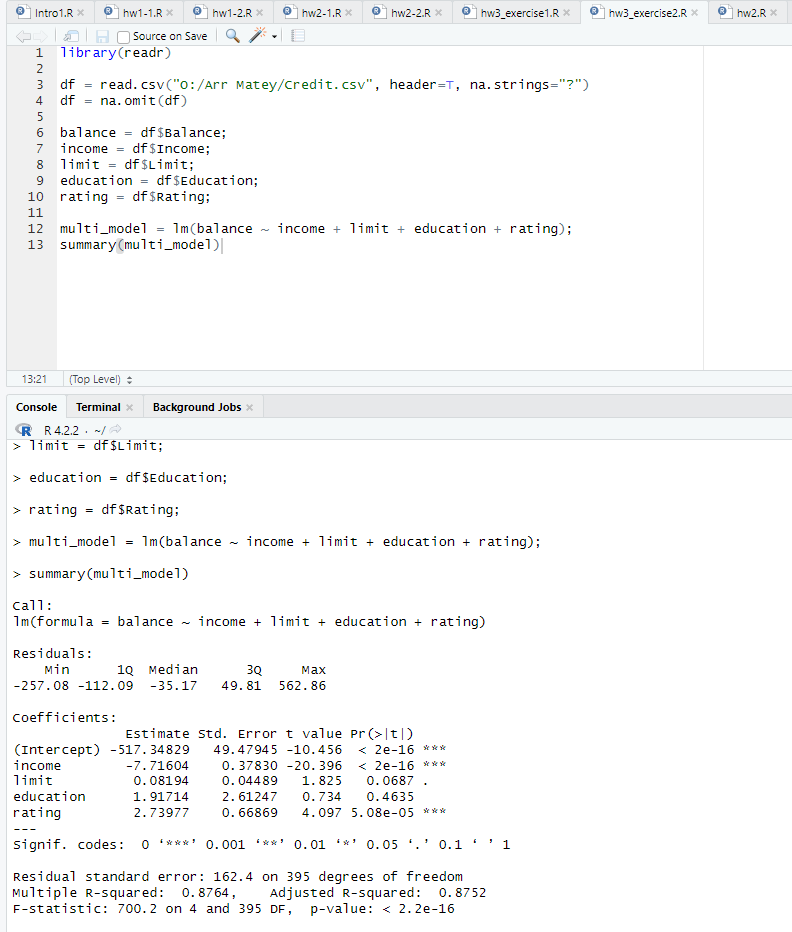
\includegraphics[width=6in]{img/ex2.PNG}
\end{center}
\item Write out the estimated model in equation form.

\soln* For $i := \text{income},\; l := \text{limit},\; e := \text{education},\; r:= \text{rating}$, $$\yhat(i,l,e,r) = -517.34829 - 7.71604i + 0.08194l + 1.91714e + 2.73977r$$
\item Provide the interpretation of each coefficient in the model.

\soln* The intercept of $-517.34829$ means that at $\yhat(\vec{0})$ (all variables zero) the expected balance is $-\$517.35$.

\nl For every unit increase of income, the expected value of balance drops by 7.71604.

\nl For every unit increase of limit, the expected value of balance increases by 0.08194.

\nl For every unit increase of education, the expected value of balance increases by 1.91714.

\nl For every unit increase of rating, the expected value of balance increases by 2.73977.
\item Obtain 95\% confidence intervals for the coefficient(s)

\soln*
\begin{center}
    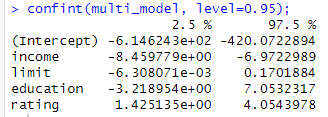
\includegraphics[width=4in]{img/ex2d.PNG}
\end{center}
With 95\% confidence, the coefficients' intervals are
\begin{itemize}
    \item Intercept: $(-\$420.07,\,-\$614.62)$
    \item Income: $(-\$8.46,\,-\$6.97)$
    \item Limit: $(-\$0.006,\,\$0.17)$
    \item Education: $(-\$3.22,\,\$7.05)$
    \item Rating: $(\$1.43,\,\$4.05)$
\end{itemize}



\item Test whether all the regression coefficients are zero (there is a linear relationship
between the response and the predictors), i.e whether $\bat_1 = \bat_2 = \bat_3 = \bat_4 = 0$.

\soln* Based on the model summary, since $p = 2.2 \cdot 10^{-16} < 0.05 = \alpha$, there is sufficient evidence that all of the predictor variables are significant (non zero).
\item Based on the $p$-values in part (a), which predictor(s) seem(s) to not have an
association with the response variable (\green{Balance})

\soln* The predictors Limit and Education seem to not be associated with Balance because their $p$-values are greater than $\alpha$ (0.0687 and 0.4635 respectively).
\item On the basis of your response to the previous question, fit a smaller model that only
uses the predictors for which there is evidence of association with the response variable.

\soln* $\yhat(i,r) = -534.81215 - 7.67212i + 3.94926 r $
\begin{center}
    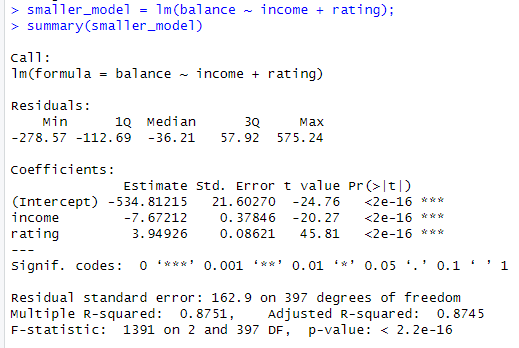
\includegraphics[width=6in]{img/ex2g.PNG}
\end{center}
\item Test whether the coefficients of the predictor(s) in (f) are all zero. Would you drop
those predictors from the full model? Why?

\soln* $H_0 : \bat_l = \bat_e = 0$ versus $H_a : \bat_l \neq 0 \lor \bat_e \neq 0$.
\\(next page)
\begin{center}
    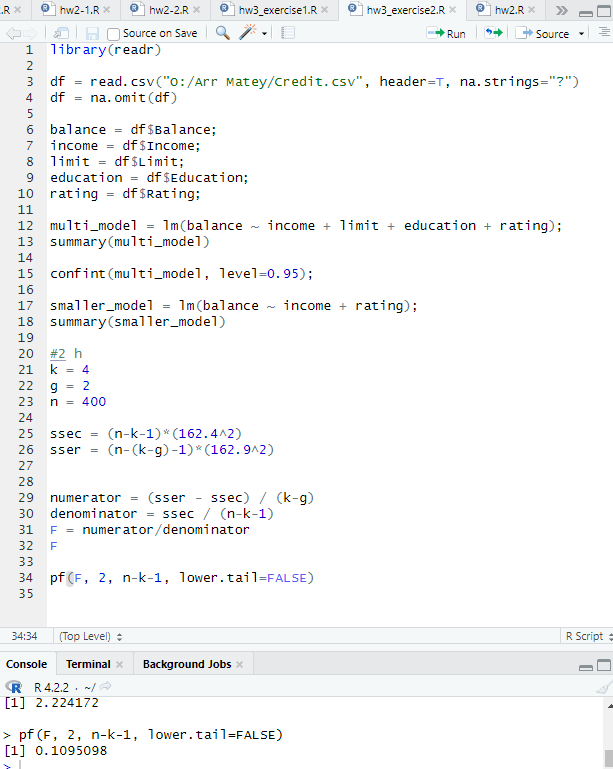
\includegraphics[width=6in]{img/ex2h.PNG}
\end{center}

Since $p = 0.1095 \not < \alpha = 0.05$, we fail to reject $H_0$. Hence there is not enough evidence to indicate a relationship between the predictors limit and education with response balance. Therefore I would remove these the full model, especially since income and rating have over a 99\% significance. 
\end{enumerate}

\end{enumerate}

\end{document}
